% $Header: /u/gcmpack/manual/s_algorithm/text/tracer.tex,v 1.25 2010/08/27 13:08:18 jmc Exp $
% $Name:  $

\section{Tracer equations}
\label{sect:tracer_equations}
\begin{rawhtml}
<!-- CMIREDIR:tracer_equations: -->
\end{rawhtml}

The basic discretization used for the tracer equations is the second
order piece-wise constant finite volume form of the forced
advection-diffusion equations. There are many alternatives to second
order method for advection and alternative parameterizations for the
sub-grid scale processes. The Gent-McWilliams eddy parameterization,
KPP mixing scheme and PV flux parameterization are all dealt with in
separate sections. The basic discretization of the advection-diffusion
part of the tracer equations and the various advection schemes will be
described here.

\subsection{Time-stepping of tracers: ABII}
\label{sect:tracer_equations_abII}
\begin{rawhtml}
<!-- CMIREDIR:tracer_equations_abII: -->
\end{rawhtml}

The default advection scheme is the centered second order method which
requires a second order or quasi-second order time-stepping scheme to
be stable. Historically this has been the quasi-second order
Adams-Bashforth method (ABII) and applied to all terms. For an
arbitrary tracer, $\tau$, the forced advection-diffusion equation
reads:
\begin{equation}
\partial_t \tau + G_{adv}^\tau = G_{diff}^\tau + G_{forc}^\tau
\end{equation}
where $G_{adv}^\tau$, $G_{diff}^\tau$ and $G_{forc}^\tau$ are the
tendencies due to advection, diffusion and forcing, respectively,
namely:
\begin{eqnarray}
G_{adv}^\tau & = & \partial_x u \tau + \partial_y v \tau + \partial_r w \tau
- \tau \nabla \cdot {\bf v} \\
G_{diff}^\tau & = & \nabla \cdot {\bf K} \nabla \tau
\end{eqnarray}
and the forcing can be some arbitrary function of state, time and
space.

The term, $\tau \nabla \cdot {\bf v}$, is required to retain local
conservation in conjunction with the linear implicit free-surface. It
only affects the surface layer since the flow is non-divergent
everywhere else. This term is therefore referred to as the surface
correction term. Global conservation is not possible using the
flux-form (as here) and a linearized free-surface
(\cite{griffies:00,campin:02}).

The continuity equation can be recovered by setting
$G_{diff}=G_{forc}=0$ and $\tau=1$.

The driver routine that calls the routines to calculate tendencies are
{\em S/R CALC\_GT} and {\em S/R CALC\_GS} for temperature and salt
(moisture), respectively. These in turn call a generic advection
diffusion routine {\em S/R GAD\_CALC\_RHS} that is called with the
flow field and relevant tracer as arguments and returns the collective
tendency due to advection and diffusion. Forcing is add subsequently
in {\em S/R CALC\_GT} or {\em S/R CALC\_GS} to the same tendency
array.

\fbox{ \begin{minipage}{4.75in}
{\em S/R GAD\_CALC\_RHS} ({\em pkg/generic\_advdiff/gad\_calc\_rhs.F})

$\tau$: {\bf tracer} (argument)

$G^{(n)}$: {\bf gTracer} (argument)

$F_r$: {\bf fVerT} (argument)

\end{minipage} }

The space and time discretization are treated separately (method of
lines). Tendencies are calculated at time levels $n$ and $n-1$ and
extrapolated to $n+1/2$ using the Adams-Bashforth method:
\marginpar{$\epsilon$: {\bf AB\_eps}}
\begin{equation}
G^{(n+1/2)} = 
(\frac{3}{2} + \epsilon) G^{(n)} - (\frac{1}{2} + \epsilon) G^{(n-1)}
\end{equation}
where $G^{(n)} = G_{adv}^\tau + G_{diff}^\tau + G_{src}^\tau$ at time
step $n$. The tendency at $n-1$ is not re-calculated but rather the
tendency at $n$ is stored in a global array for later re-use.

\fbox{ \begin{minipage}{4.75in}
{\em S/R ADAMS\_BASHFORTH2} ({\em model/src/adams\_bashforth2.F})

$G^{(n+1/2)}$: {\bf gTracer} (argument on exit)

$G^{(n)}$: {\bf gTracer} (argument on entry)

$G^{(n-1)}$: {\bf gTrNm1} (argument)

$\epsilon$: {\bf ABeps} (PARAMS.h)

\end{minipage} }

The tracers are stepped forward in time using the extrapolated tendency:
\begin{equation}
\tau^{(n+1)} = \tau^{(n)} + \Delta t G^{(n+1/2)}
\end{equation}
\marginpar{$\Delta t$: {\bf deltaTtracer}}

\fbox{ \begin{minipage}{4.75in}
{\em S/R TIMESTEP\_TRACER} ({\em model/src/timestep\_tracer.F})

$\tau^{(n+1)}$: {\bf gTracer} (argument on exit)

$\tau^{(n)}$: {\bf tracer} (argument on entry)

$G^{(n+1/2)}$: {\bf gTracer} (argument)

$\Delta t$: {\bf deltaTtracer} (PARAMS.h)

\end{minipage} }

Strictly speaking the ABII scheme should be applied only to the
advection terms. However, this scheme is only used in conjunction with
the standard second, third and fourth order advection
schemes. Selection of any other advection scheme disables
Adams-Bashforth for tracers so that explicit diffusion and forcing use
the forward method.




\section{Linear advection schemes}
\label{sect:tracer-advection}
\begin{rawhtml}
<!-- CMIREDIR:linear_advection_schemes: -->
\end{rawhtml}

\begin{figure}
\resizebox{5.5in}{!}{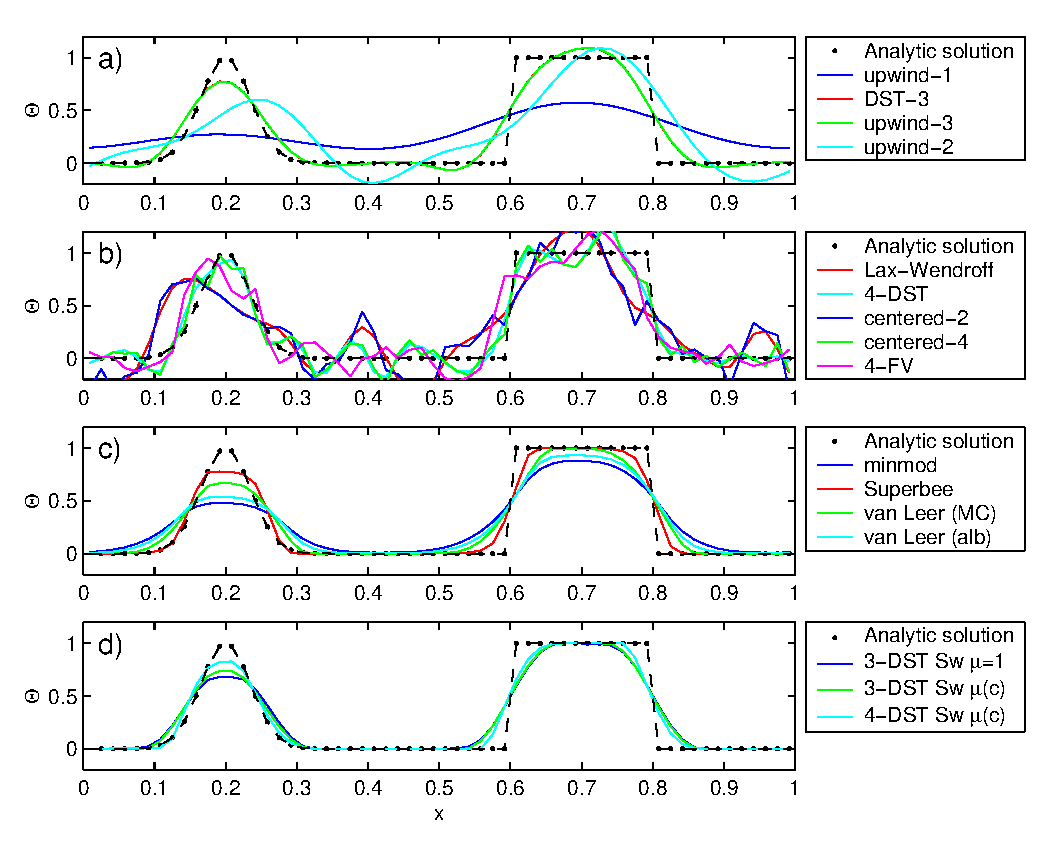
\includegraphics{s_algorithm/figs/advect-1d-lo.eps}}
\caption{
Comparison of 1-D advection schemes. Courant number is 0.05 with 60
points and solutions are shown for T=1 (one complete period).
a) Shows the upwind biased schemes; first order upwind, DST3,
third order upwind and second order upwind.
b) Shows the centered schemes; Lax-Wendroff, DST4, centered second order,
centered fourth order and finite volume fourth order.
c) Shows the second order flux limiters: minmod, Superbee,
MC limiter and the van Leer limiter.
d) Shows the DST3 method with flux limiters due to Sweby with
$\mu=1$, $\mu=c/(1-c)$ and a fourth order DST method with Sweby limiter,
$\mu=c/(1-c)$.
\label{fig:advect-1d-lo}
}
\end{figure}

\begin{figure}
\resizebox{5.5in}{!}{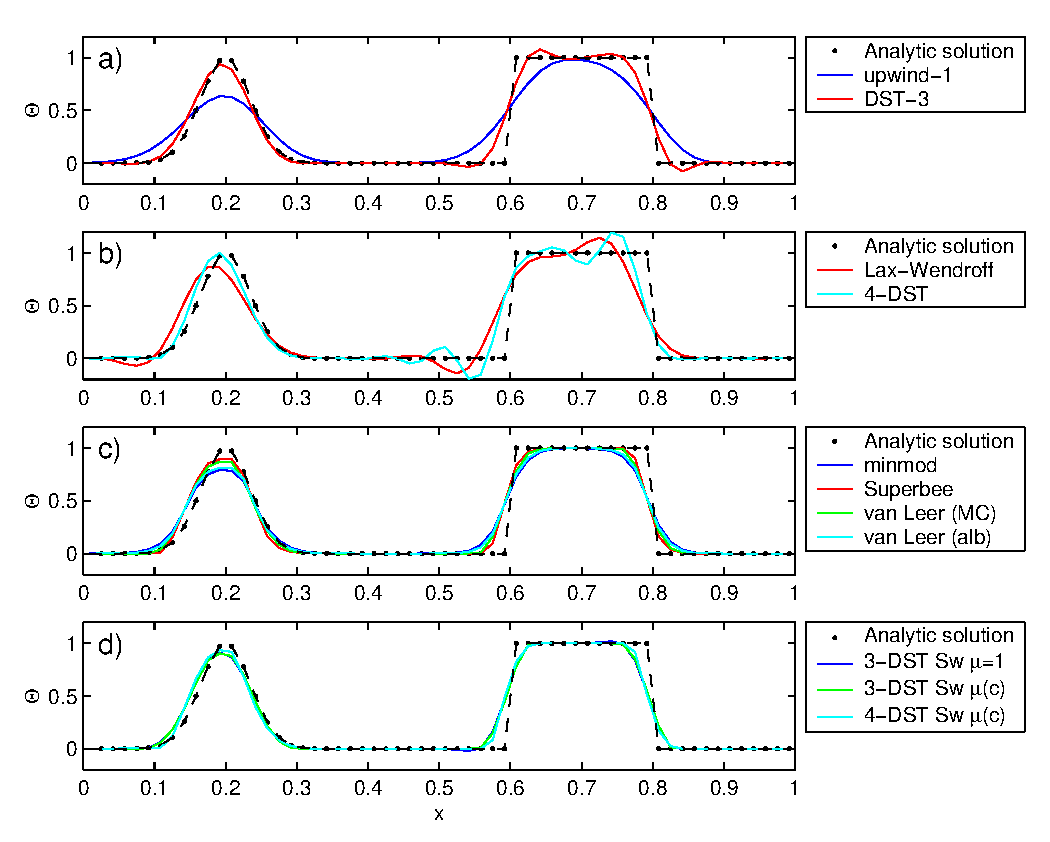
\includegraphics{s_algorithm/figs/advect-1d-hi.eps}}
\caption{
Comparison of 1-D advection schemes. Courant number is 0.89 with 60
points and solutions are shown for T=1 (one complete period).
a) Shows the upwind biased schemes; first order upwind and DST3.
Third order upwind and second order upwind are unstable at this Courant number.
b) Shows the centered schemes; Lax-Wendroff, DST4. Centered second order,
centered fourth order and finite volume fourth order and unstable at this
Courant number.
c) Shows the second order flux limiters: minmod, Superbee,
MC limiter and the van Leer limiter.
d) Shows the DST3 method with flux limiters due to Sweby with
$\mu=1$, $\mu=c/(1-c)$ and a fourth order DST method with Sweby limiter,
$\mu=c/(1-c)$.
\label{fig:advect-1d-hi}
}
\end{figure}

The advection schemes known as centered second order, centered fourth
order, first order upwind and upwind biased third order are known as
linear advection schemes because the coefficient for interpolation of
the advected tracer are linear and a function only of the flow, not
the tracer field it self. We discuss these first since they are most
commonly used in the field and most familiar.

\subsection{Centered second order advection-diffusion}

The basic discretization, centered second order, is the default. It is
designed to be consistent with the continuity equation to facilitate
conservation properties analogous to the continuum. However, centered
second order advection is notoriously noisy and must be used in
conjunction with some finite amount of diffusion to produce a sensible
solution.

The advection operator is discretized:
\begin{equation}
{\cal A}_c \Delta r_f h_c G_{adv}^\tau = 
\delta_i F_x + \delta_j F_y + \delta_k F_r
\end{equation}
where the area integrated fluxes are given by:
\begin{eqnarray}
F_x & = & U \overline{ \tau }^i \\
F_y & = & V \overline{ \tau }^j \\
F_r & = & W \overline{ \tau }^k
\end{eqnarray}
The quantities $U$, $V$ and $W$ are volume fluxes defined:
\marginpar{$U$: {\bf uTrans} }
\marginpar{$V$: {\bf vTrans} }
\marginpar{$W$: {\bf rTrans} }
\begin{eqnarray}
U & = & \Delta y_g \Delta r_f h_w u \\
V & = & \Delta x_g \Delta r_f h_s v \\
W & = & {\cal A}_c w
\end{eqnarray}

For non-divergent flow, this discretization can be shown to conserve
the tracer both locally and globally and to globally conserve tracer
variance, $\tau^2$. The proof is given in \cite{adcroft:95,adcroft:97}.

\fbox{ \begin{minipage}{4.75in}
{\em S/R GAD\_C2\_ADV\_X} ({\em gad\_c2\_adv\_x.F})

$F_x$: {\bf uT} (argument)

$U$: {\bf uTrans} (argument)

$\tau$: {\bf tracer} (argument)

{\em S/R GAD\_C2\_ADV\_Y} ({\em gad\_c2\_adv\_y.F})

$F_y$: {\bf vT} (argument)

$V$: {\bf vTrans} (argument)

$\tau$: {\bf tracer} (argument)

{\em S/R GAD\_C2\_ADV\_R} ({\em gad\_c2\_adv\_r.F})

$F_r$: {\bf wT} (argument)

$W$: {\bf rTrans} (argument)

$\tau$: {\bf tracer} (argument)

\end{minipage} }


\subsection{Third order upwind bias advection}

Upwind biased third order advection offers a relatively good
compromise between accuracy and smoothness. It is not a ``positive''
scheme meaning false extrema are permitted but the amplitude of such
are significantly reduced over the centered second order method.

The third order upwind fluxes are discretized:
\begin{eqnarray}
F_x & = & U \overline{\tau - \frac{1}{6} \delta_{ii} \tau}^i
         + \frac{1}{2} |U| \delta_i \frac{1}{6} \delta_{ii} \tau \\
F_y & = & V \overline{\tau - \frac{1}{6} \delta_{ii} \tau}^j
         + \frac{1}{2} |V| \delta_j \frac{1}{6} \delta_{jj} \tau \\
F_r & = & W \overline{\tau - \frac{1}{6} \delta_{ii} \tau}^k
         + \frac{1}{2} |W| \delta_k \frac{1}{6} \delta_{kk} \tau 
\end{eqnarray}

At boundaries, $\delta_{\hat{n}} \tau$ is set to zero allowing
$\delta_{nn}$ to be evaluated. We are currently examine the accuracy
of this boundary condition and the effect on the solution.

\fbox{ \begin{minipage}{4.75in}
{\em S/R GAD\_U3\_ADV\_X} ({\em gad\_u3\_adv\_x.F})

$F_x$: {\bf uT} (argument)

$U$: {\bf uTrans} (argument)

$\tau$: {\bf tracer} (argument)

{\em S/R GAD\_U3\_ADV\_Y} ({\em gad\_u3\_adv\_y.F})

$F_y$: {\bf vT} (argument)

$V$: {\bf vTrans} (argument)

$\tau$: {\bf tracer} (argument)

{\em S/R GAD\_U3\_ADV\_R} ({\em gad\_u3\_adv\_r.F})

$F_r$: {\bf wT} (argument)

$W$: {\bf rTrans} (argument)

$\tau$: {\bf tracer} (argument)

\end{minipage} }

\subsection{Centered fourth order advection}

Centered fourth order advection is formally the most accurate scheme
we have implemented and can be used to great effect in high resolution
simulation where dynamical scales are well resolved. However, the
scheme is noisy like the centered second order method and so must be
used with some finite amount of diffusion. Bi-harmonic is recommended
since it is more scale selective and less likely to diffuse away the
well resolved gradient the fourth order scheme worked so hard to
create.

The centered fourth order fluxes are discretized:
\begin{eqnarray}
F_x & = & U \overline{\tau - \frac{1}{6} \delta_{ii} \tau}^i \\
F_y & = & V \overline{\tau - \frac{1}{6} \delta_{ii} \tau}^j \\
F_r & = & W \overline{\tau - \frac{1}{6} \delta_{ii} \tau}^k
\end{eqnarray}

As for the third order scheme, the best discretization near boundaries
is under investigation but currently $\delta_i \tau=0$ on a boundary.

\fbox{ \begin{minipage}{4.75in}
{\em S/R GAD\_C4\_ADV\_X} ({\em gad\_c4\_adv\_x.F})

$F_x$: {\bf uT} (argument)

$U$: {\bf uTrans} (argument)

$\tau$: {\bf tracer} (argument)

{\em S/R GAD\_C4\_ADV\_Y} ({\em gad\_c4\_adv\_y.F})

$F_y$: {\bf vT} (argument)

$V$: {\bf vTrans} (argument)

$\tau$: {\bf tracer} (argument)

{\em S/R GAD\_C4\_ADV\_R} ({\em gad\_c4\_adv\_r.F})

$F_r$: {\bf wT} (argument)

$W$: {\bf rTrans} (argument)

$\tau$: {\bf tracer} (argument)

\end{minipage} }


\subsection{First order upwind advection}

Although the upwind scheme is the underlying scheme for the robust or
non-linear methods given later, we haven't actually supplied this
method for general use. It would be very diffusive and it is unlikely
that it could ever produce more useful results than the positive
higher order schemes.

Upwind bias is introduced into many schemes using the {\em abs}
function and is allows the first order upwind flux to be written:
\begin{eqnarray}
F_x & = & U \overline{ \tau }^i - \frac{1}{2} |U| \delta_i \tau \\
F_y & = & V \overline{ \tau }^j - \frac{1}{2} |V| \delta_j \tau \\
F_r & = & W \overline{ \tau }^k - \frac{1}{2} |W| \delta_k \tau
\end{eqnarray}

If for some reason, the above method is required, then the second
order flux limiter scheme described later reduces to the above scheme
if the limiter is set to zero.


\section{Non-linear advection schemes}
\label{sect:non-linear_advection_schemes}
\begin{rawhtml}
<!-- CMIREDIR:non-linear_advection_schemes: -->
\end{rawhtml}

Non-linear advection schemes invoke non-linear interpolation and are
widely used in computational fluid dynamics (non-linear does not refer
to the non-linearity of the advection operator). The flux limited
advection schemes belong to the class of finite volume methods which
neatly ties into the spatial discretization of the model.

When employing the flux limited schemes, first order upwind or
direct-space-time method the time-stepping is switched to forward in
time.

\subsection{Second order flux limiters}

The second order flux limiter method can be cast in several ways but
is generally expressed in terms of other flux approximations. For
example, in terms of a first order upwind flux and second order
Lax-Wendroff flux, the limited flux is given as:
\begin{equation}
F = F_1 + \psi(r) F_{LW}
\end{equation}
where $\psi(r)$ is the limiter function,
\begin{equation}
F_1 = u \overline{\tau}^i - \frac{1}{2} |u| \delta_i \tau
\end{equation}
is the upwind flux,
\begin{equation}
F_{LW} = F_1 + \frac{|u|}{2} (1-c) \delta_i \tau
\end{equation}
is the Lax-Wendroff flux and $c = \frac{u \Delta t}{\Delta x}$ is the
Courant (CFL) number.

The limiter function, $\psi(r)$, takes the slope ratio
\begin{eqnarray}
r = \frac{ \tau_{i-1} - \tau_{i-2} }{ \tau_{i} - \tau_{i-1} } & \forall & u > 0
\\
r = \frac{ \tau_{i+1} - \tau_{i} }{ \tau_{i} - \tau_{i-1} } & \forall & u < 0
\end{eqnarray}
as it's argument. There are many choices of limiter function but we
only provide the Superbee limiter \cite{roe:85}:
\begin{equation}
\psi(r) = \max[0,\min[1,2r],\min[2,r]]
\end{equation}

\fbox{ \begin{minipage}{4.75in}
{\em S/R GAD\_FLUXLIMIT\_ADV\_X} ({\em gad\_fluxlimit\_adv\_x.F})

$F_x$: {\bf uT} (argument)

$U$: {\bf uTrans} (argument)

$\tau$: {\bf tracer} (argument)

{\em S/R GAD\_FLUXLIMIT\_ADV\_Y} ({\em gad\_fluxlimit\_adv\_y.F})

$F_y$: {\bf vT} (argument)

$V$: {\bf vTrans} (argument)

$\tau$: {\bf tracer} (argument)

{\em S/R GAD\_FLUXLIMIT\_ADV\_R} ({\em gad\_fluxlimit\_adv\_r.F})

$F_r$: {\bf wT} (argument)

$W$: {\bf rTrans} (argument)

$\tau$: {\bf tracer} (argument)

\end{minipage} }


\subsection{Third order direct space time}

The direct-space-time method deals with space and time discretization
together (other methods that treat space and time separately are known
collectively as the ``Method of Lines''). The Lax-Wendroff scheme
falls into this category; it adds sufficient diffusion to a second
order flux that the forward-in-time method is stable. The upwind
biased third order DST scheme is:
\begin{eqnarray}
F = u \left( \tau_{i-1}
        + d_0 (\tau_{i}-\tau_{i-1}) + d_1 (\tau_{i-1}-\tau_{i-2}) \right)
& \forall & u > 0 \\
F = u \left( \tau_{i}
        - d_0 (\tau_{i}-\tau_{i-1}) - d_1 (\tau_{i+1}-\tau_{i}) \right)
& \forall & u < 0
\end{eqnarray}
where
\begin{eqnarray}
d_1 & = & \frac{1}{6} ( 2 - |c| ) ( 1 - |c| ) \\
d_2 & = & \frac{1}{6} ( 1 - |c| ) ( 1 + |c| )
\end{eqnarray}
The coefficients $d_0$ and $d_1$ approach $1/3$ and $1/6$ respectively
as the Courant number, $c$, vanishes. In this limit, the conventional
third order upwind method is recovered. For finite Courant number, the
deviations from the linear method are analogous to the diffusion added
to centered second order advection in the Lax-Wendroff scheme.

The DST3 method described above must be used in a forward-in-time
manner and is stable for $0 \le |c| \le 1$. Although the scheme
appears to be forward-in-time, it is in fact third order in time and
the accuracy increases with the Courant number! For low Courant
number, DST3 produces very similar results (indistinguishable in
Fig.~\ref{fig:advect-1d-lo}) to the linear third order method but for
large Courant number, where the linear upwind third order method is
unstable, the scheme is extremely accurate
(Fig.~\ref{fig:advect-1d-hi}) with only minor overshoots.

\fbox{ \begin{minipage}{4.75in}
{\em S/R GAD\_DST3\_ADV\_X} ({\em gad\_dst3\_adv\_x.F})

$F_x$: {\bf uT} (argument)

$U$: {\bf uTrans} (argument)

$\tau$: {\bf tracer} (argument)

{\em S/R GAD\_DST3\_ADV\_Y} ({\em gad\_dst3\_adv\_y.F})

$F_y$: {\bf vT} (argument)

$V$: {\bf vTrans} (argument)

$\tau$: {\bf tracer} (argument)

{\em S/R GAD\_DST3\_ADV\_R} ({\em gad\_dst3\_adv\_r.F})

$F_r$: {\bf wT} (argument)

$W$: {\bf rTrans} (argument)

$\tau$: {\bf tracer} (argument)

\end{minipage} }


\subsection{Third order direct space time with flux limiting}

The overshoots in the DST3 method can be controlled with a flux limiter.
The limited flux is written:
\begin{equation}
F =
\frac{1}{2}(u+|u|)\left( \tau_{i-1} + \psi(r^+)(\tau_{i} - \tau_{i-1} )\right)
+
\frac{1}{2}(u-|u|)\left( \tau_{i-1} + \psi(r^-)(\tau_{i} - \tau_{i-1} )\right)
\end{equation}
where
\begin{eqnarray}
r^+ & = & \frac{\tau_{i-1} - \tau_{i-2}}{\tau_{i} - \tau_{i-1}} \\
r^- & = & \frac{\tau_{i+1} - \tau_{i}}{\tau_{i} - \tau_{i-1}}
\end{eqnarray}
and the limiter is the Sweby limiter:
\begin{equation}
\psi(r) = \max[0, \min[\min(1,d_0+d_1r],\frac{1-c}{c}r ]]
\end{equation}

\fbox{ \begin{minipage}{4.75in}
{\em S/R GAD\_DST3FL\_ADV\_X} ({\em gad\_dst3\_adv\_x.F})

$F_x$: {\bf uT} (argument)

$U$: {\bf uTrans} (argument)

$\tau$: {\bf tracer} (argument)

{\em S/R GAD\_DST3FL\_ADV\_Y} ({\em gad\_dst3\_adv\_y.F})

$F_y$: {\bf vT} (argument)

$V$: {\bf vTrans} (argument)

$\tau$: {\bf tracer} (argument)

{\em S/R GAD\_DST3FL\_ADV\_R} ({\em gad\_dst3\_adv\_r.F})

$F_r$: {\bf wT} (argument)

$W$: {\bf rTrans} (argument)

$\tau$: {\bf tracer} (argument)

\end{minipage} }


\subsection{Multi-dimensional advection}

\begin{figure}
\resizebox{5.5in}{!}{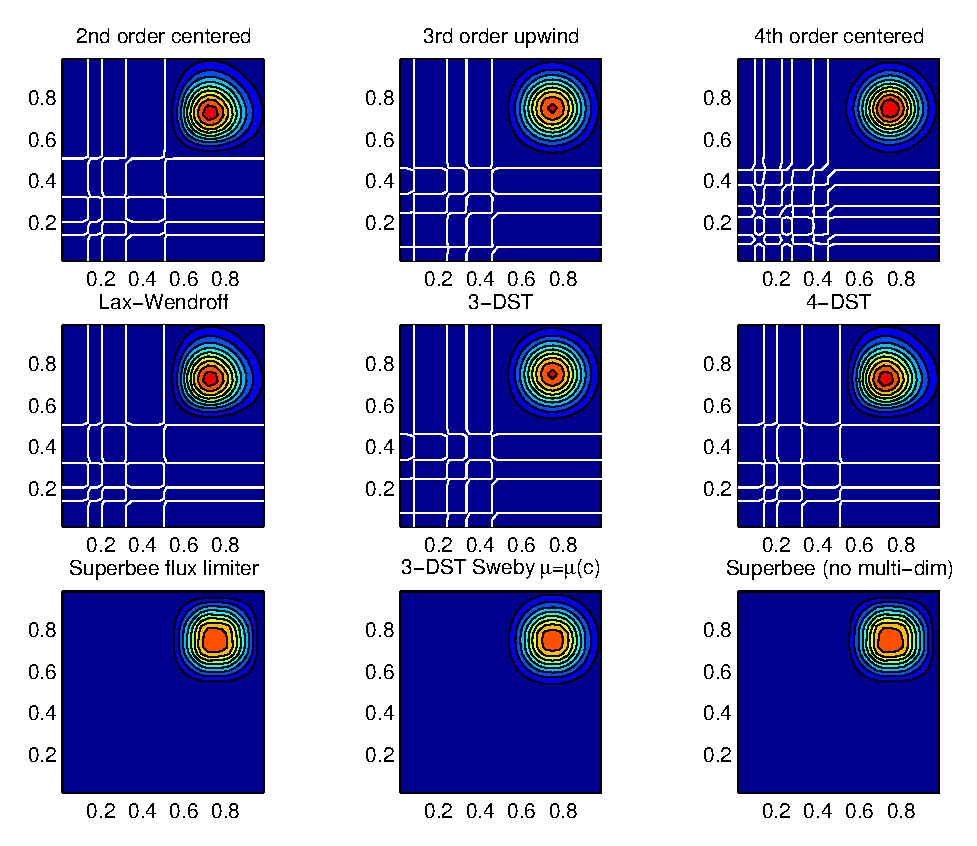
\includegraphics{s_algorithm/figs/advect-2d-lo-diag.eps}}
\caption{
Comparison of advection schemes in two dimensions; diagonal advection
of a resolved Gaussian feature. Courant number is 0.01 with
30$\times$30 points and solutions are shown for T=1/2. White lines
indicate zero crossing (ie. the presence of false minima).  The left
column shows the second order schemes; top) centered second order with
Adams-Bashforth, middle) Lax-Wendroff and bottom) Superbee flux
limited. The middle column shows the third order schemes; top) upwind
biased third order with Adams-Bashforth, middle) third order direct
space-time method and bottom) the same with flux limiting. The top
right panel shows the centered fourth order scheme with
Adams-Bashforth and right middle panel shows a fourth order variant on
the DST method. Bottom right panel shows the Superbee flux limiter
(second order) applied independently in each direction (method of
lines).
\label{fig:advect-2d-lo-diag}
}
\end{figure}

\begin{figure}
\resizebox{5.5in}{!}{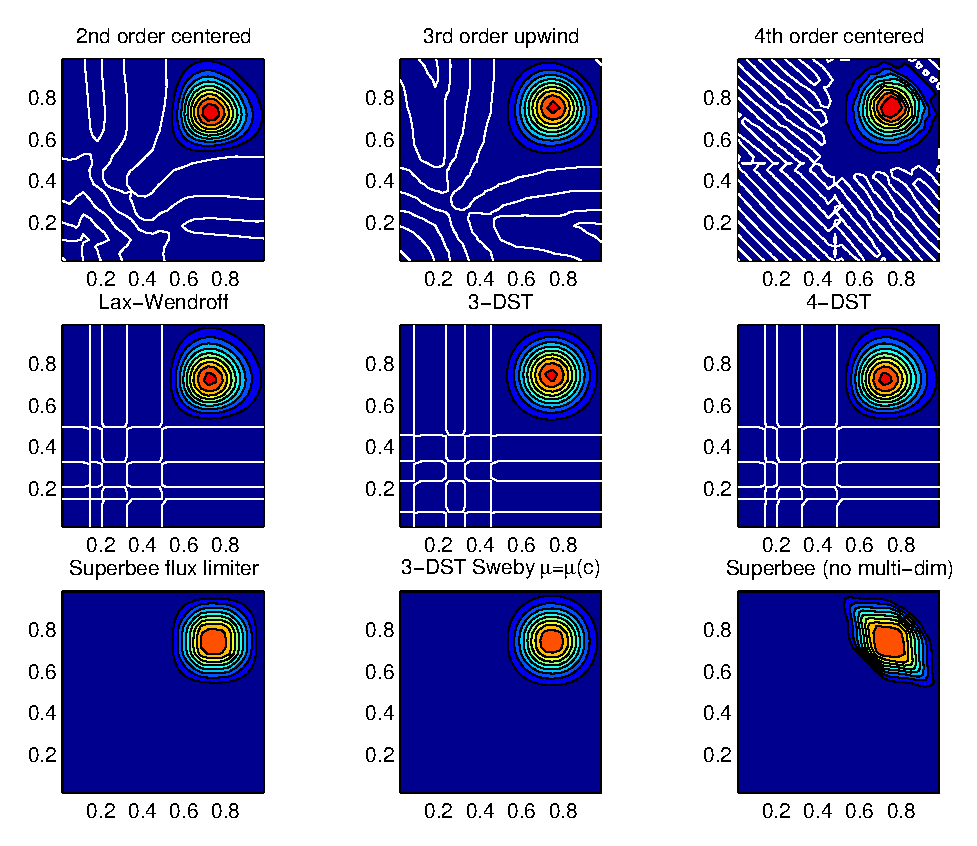
\includegraphics{s_algorithm/figs/advect-2d-mid-diag.eps}}
\caption{
Comparison of advection schemes in two dimensions; diagonal advection
of a resolved Gaussian feature. Courant number is 0.27 with
30$\times$30 points and solutions are shown for T=1/2. White lines
indicate zero crossing (ie. the presence of false minima).  The left
column shows the second order schemes; top) centered second order with
Adams-Bashforth, middle) Lax-Wendroff and bottom) Superbee flux
limited. The middle column shows the third order schemes; top) upwind
biased third order with Adams-Bashforth, middle) third order direct
space-time method and bottom) the same with flux limiting. The top
right panel shows the centered fourth order scheme with
Adams-Bashforth and right middle panel shows a fourth order variant on
the DST method. Bottom right panel shows the Superbee flux limiter
(second order) applied independently in each direction (method of
lines).
\label{fig:advect-2d-mid-diag}
}
\end{figure}

\begin{figure}
\resizebox{5.5in}{!}{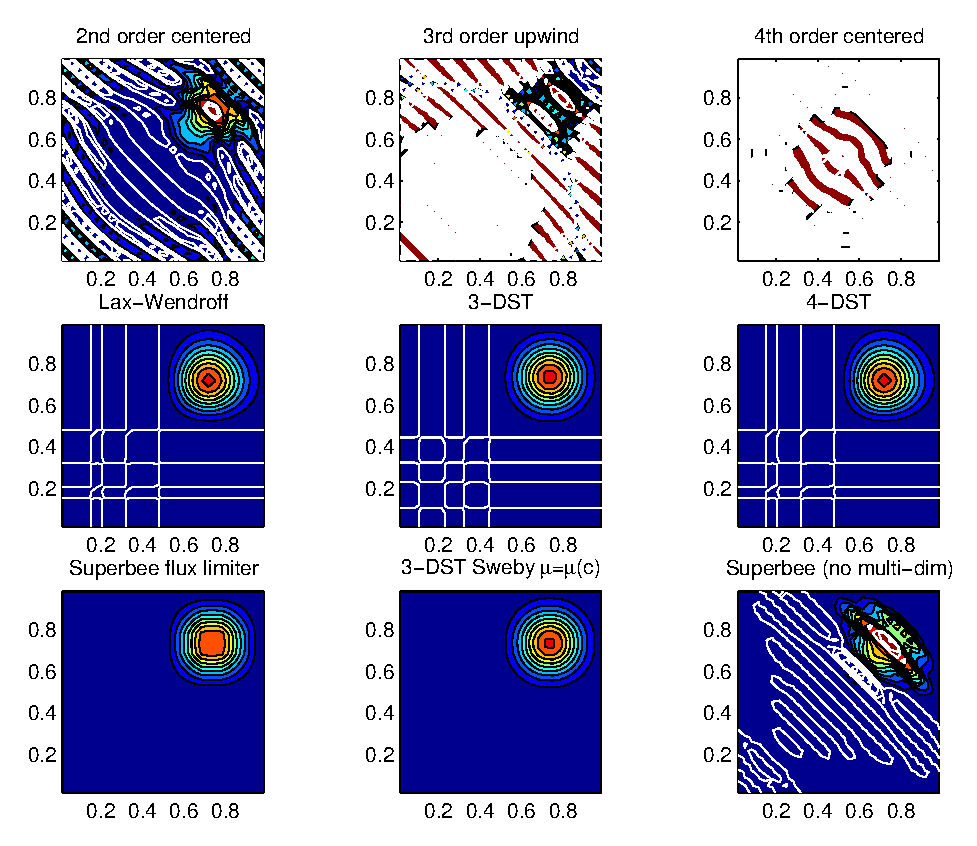
\includegraphics{s_algorithm/figs/advect-2d-hi-diag.eps}}
\caption{
Comparison of advection schemes in two dimensions; diagonal advection
of a resolved Gaussian feature. Courant number is 0.47 with
30$\times$30 points and solutions are shown for T=1/2. White lines
indicate zero crossings and initial maximum values (ie. the presence
of false extrema).  The left column shows the second order schemes;
top) centered second order with Adams-Bashforth, middle) Lax-Wendroff
and bottom) Superbee flux limited. The middle column shows the third
order schemes; top) upwind biased third order with Adams-Bashforth,
middle) third order direct space-time method and bottom) the same with
flux limiting. The top right panel shows the centered fourth order
scheme with Adams-Bashforth and right middle panel shows a fourth
order variant on the DST method. Bottom right panel shows the Superbee
flux limiter (second order) applied independently in each direction
(method of lines).
\label{fig:advect-2d-hi-diag}
}
\end{figure}



In many of the aforementioned advection schemes the behavior in
multiple dimensions is not necessarily as good as the one dimensional
behavior. For instance, a shape preserving monotonic scheme in one
dimension can have severe shape distortion in two dimensions if the
two components of horizontal fluxes are treated independently. There
is a large body of literature on the subject dealing with this problem
and among the fixes are operator and flux splitting methods, corner
flux methods and more. We have adopted a variant on the standard
splitting methods that allows the flux calculations to be implemented
as if in one dimension:
\begin{eqnarray}
\tau^{n+1/3} & = & \tau^{n}
- \Delta t \left( \frac{1}{\Delta x} \delta_i F^x(\tau^{n})
           + \tau^{n} \frac{1}{\Delta x} \delta_i u \right) \\
\tau^{n+2/3} & = & \tau^{n+1/3}
- \Delta t \left( \frac{1}{\Delta y} \delta_j F^y(\tau^{n+1/3})
           + \tau^{n} \frac{1}{\Delta y} \delta_i v \right) \\
\tau^{n+3/3} & = & \tau^{n+2/3}
- \Delta t \left( \frac{1}{\Delta r} \delta_k F^x(\tau^{n+2/3})
           + \tau^{n} \frac{1}{\Delta r} \delta_i w \right)
\end{eqnarray}

In order to incorporate this method into the general model algorithm,
we compute the effective tendency rather than update the tracer so
that other terms such as diffusion are using the $n$ time-level and
not the updated $n+3/3$ quantities:
\begin{equation}
G^{n+1/2}_{adv} = \frac{1}{\Delta t} ( \tau^{n+3/3} - \tau^{n} )
\end{equation}
So that the over all time-stepping looks likes:
\begin{equation}
\tau^{n+1} = \tau^{n} + \Delta t \left( G^{n+1/2}_{adv} + G_{diff}(\tau^{n}) + G^{n}_{forcing} \right)
\end{equation}

\fbox{ \begin{minipage}{4.75in}
{\em S/R GAD\_ADVECTION} ({\em gad\_advection.F})

$\tau$: {\bf Tracer} (argument)

$G^{n+1/2}_{adv}$: {\bf Gtracer} (argument)

$F_x, F_y, F_r$: {\bf af} (local)

$U$: {\bf uTrans} (local)

$V$: {\bf vTrans} (local)

$W$: {\bf rTrans} (local)

\end{minipage} }

\begin{figure}
\resizebox{3.5in}{!}{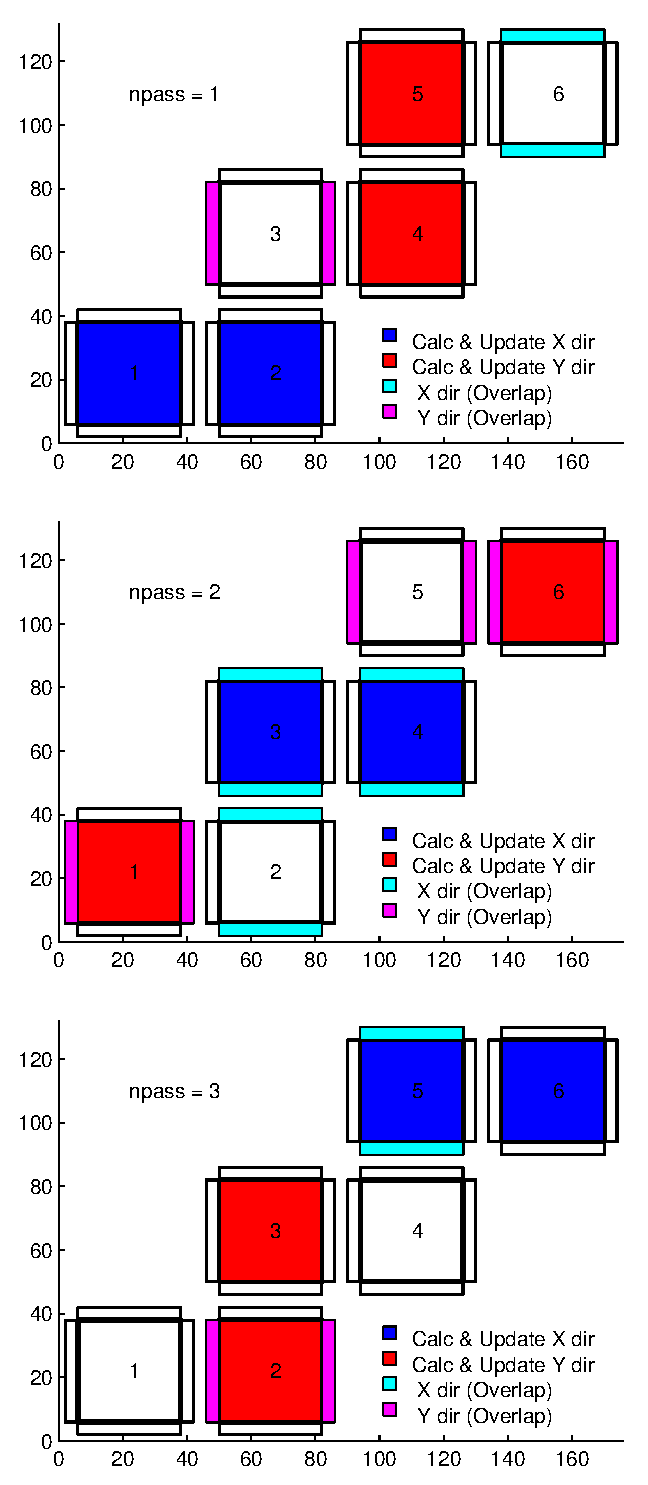
\includegraphics{s_algorithm/figs/multiDim_CS.eps}}
\caption{Muti-dimensional advection time-stepping with Cubed-Sphere topology
\label{fig:advect-multidim_cs}
}
\end{figure}

\section{Comparison of advection schemes}
\label{sect:tracer_advection_schemes}
\begin{rawhtml}
<!-- CMIREDIR:comparison_of_advection_schemes: -->
\end{rawhtml}

\begin{table}[htb]
\centering
 \begin{tabular}[htb]{|l|c|c|c|c|l|}
   \hline
   Advection Scheme & code & use  & use Multi- & Stencil & comments \\
                    &      & A.B. & dimension & (1 dim) & \\
   \hline \hline
   $1^{rst}$order upwind  & 1 &  No & Yes & 3 pts & linear/$\tau$, non-linear/v\\
   \hline
   centered $2^{nd}$order & 2 &  Yes & No & 3 pts & linear \\
   \hline
   $3^{rd}$order upwind   & 3 &  Yes & No & 5 pts & linear/$\tau$\\
   \hline
   centered $4^{th}$order & 4 &  Yes & No & 5 pts & linear \\
   \hline \hline
   $2^{nd}$order DST (Lax-Wendroff)  & 20 &
                         No & Yes & 3 pts & linear/$\tau$, non-linear/v\\
   \hline
   $3^{rd}$order DST & 30 &  No & Yes & 5 pts & linear/$\tau$, non-linear/v\\
   \hline \hline
   $2^{nd}$order Flux Limiters & 77 &  No & Yes & 5 pts & non-linear \\
   \hline
   $3^{nd}$order DST Flux limiter & 33 &  No & Yes & 5 pts & non-linear \\
   \hline
 \end{tabular}
 \caption{Summary of the different advection schemes available in MITgcm.
          ``A.B.'' stands for Adams-Bashforth and ``DST'' for direct space time.
          The code corresponds to the number used to select the corresponding
          advection scheme in the parameter file (e.g., {\bf tempAdvScheme}=3 in
          file {\em data} selects the $3^{rd}$ order upwind advection scheme 
          for temperature).
   }
 \label{tab:advectionShemes_summary}
\end{table}


Figs.~\ref{fig:advect-2d-lo-diag}, \ref{fig:advect-2d-mid-diag} and
\ref{fig:advect-2d-hi-diag} show solutions to a simple diagonal
advection problem using a selection of schemes for low, moderate and
high Courant numbers, respectively. The top row shows the linear
schemes, integrated with the Adams-Bashforth method. Theses schemes
are clearly unstable for the high Courant number and weakly unstable
for the moderate Courant number. The presence of false extrema is very
apparent for all Courant numbers. The middle row shows solutions
obtained with the unlimited but multi-dimensional schemes. These
solutions also exhibit false extrema though the pattern now shows
symmetry due to the multi-dimensional scheme. Also, the schemes are
stable at high Courant number where the linear schemes weren't. The
bottom row (left and middle) shows the limited schemes and most
obvious is the absence of false extrema. The accuracy and stability of
the unlimited non-linear schemes is retained at high Courant number
but at low Courant number the tendency is to loose amplitude in sharp
peaks due to diffusion. The one dimensional tests shown in
Figs.~\ref{fig:advect-1d-lo} and \ref{fig:advect-1d-hi} showed this
phenomenon.

Finally, the bottom left and right panels use the same advection
scheme but the right does not use the multi-dimensional method. At low
Courant number this appears to not matter but for moderate Courant
number severe distortion of the feature is apparent. Moreover, the
stability of the multi-dimensional scheme is determined by the maximum
Courant number applied of each dimension while the stability of the
method of lines is determined by the sum. Hence, in the high Courant
number plot, the scheme is unstable.

With many advection schemes implemented in the code two questions
arise: ``Which scheme is best?'' and ``Why don't you just offer the
best advection scheme?''. Unfortunately, no one advection scheme is
``the best'' for all particular applications and for new applications
it is often a matter of trial to determine which is most
suitable. Here are some guidelines but these are not the rule;
\begin{itemize}
\item If you have a coarsely resolved model, using a
positive or upwind biased scheme will introduce significant diffusion
to the solution and using a centered higher order scheme will
introduce more noise. In this case, simplest may be best.
\item If you have a high resolution model, using a higher order
scheme will give a more accurate solution but scale-selective
diffusion might need to be employed. The flux limited methods
offer similar accuracy in this regime.
\item If your solution has shocks or propagating fronts then a
flux limited scheme is almost essential.
\item If your time-step is limited by advection, the multi-dimensional
non-linear schemes have the most stability (up to Courant number 1).
\item If you need to know how much diffusion/dissipation has occurred you
will have a lot of trouble figuring it out with a non-linear method.
\item The presence of false extrema is non-physical and this alone is the
strongest argument for using a positive scheme.
\end{itemize}
